\documentclass{article}
\usepackage{pgfplots}

\begin{document}

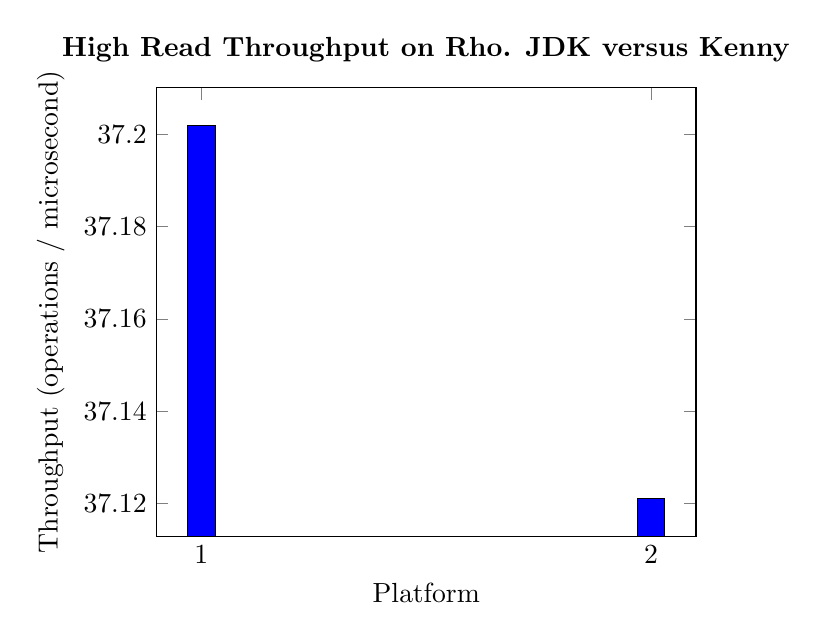
\begin{tikzpicture}
\begin{axis}[
    symbolic x coords={1,2,3,4},
    xtick=data,xlabel=Platform,ylabel=Throughput (operations / microsecond), title=\textbf{High Read Throughput on Rho. JDK versus Kenny}]
    \addplot[ybar,fill=blue] coordinates {
        (1,37.202)
        (2,37.121)
    };
\end{axis}
\end{tikzpicture}
\vspace{1cm}\\
1: My Structure\\
2: JDK Structure\\

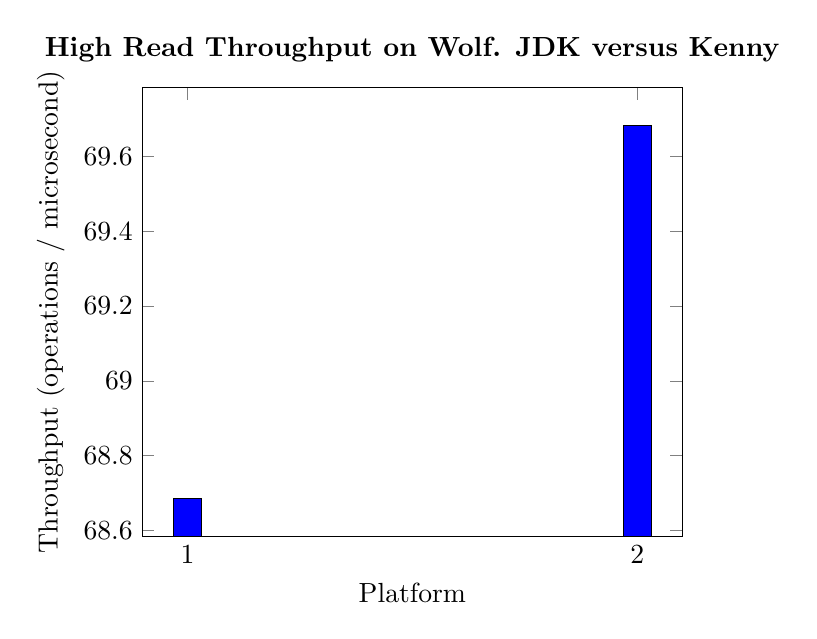
\begin{tikzpicture}
\begin{axis}[
    symbolic x coords={1,2,3,4},
    xtick=data,xlabel=Platform,ylabel=Throughput (operations / microsecond), title=\textbf{High Read Throughput on Wolf. JDK versus Kenny}]
    \addplot[ybar,fill=blue] coordinates {
        (1,68.684)
        (2,69.684)
    };
\end{axis}
\end{tikzpicture}
\vspace{1cm}\\
1: My Structure\\
2: JDK Structure\\

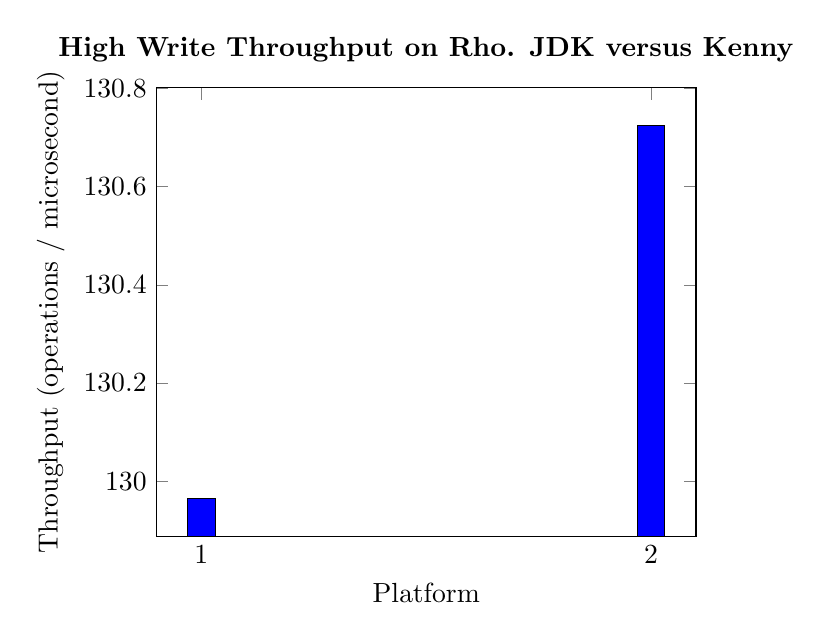
\begin{tikzpicture}
\begin{axis}[
    symbolic x coords={1,2,3,4},
    xtick=data,xlabel=Platform,ylabel=Throughput (operations / microsecond), title=\textbf{High Write Throughput on Rho. JDK versus Kenny}]
    \addplot[ybar,fill=blue] coordinates {
        (1,129.964)
        (2,130.725)
    };
\end{axis}
\end{tikzpicture}
\vspace{1cm}\\
1: My Structure\\
2: JDK Structure\\

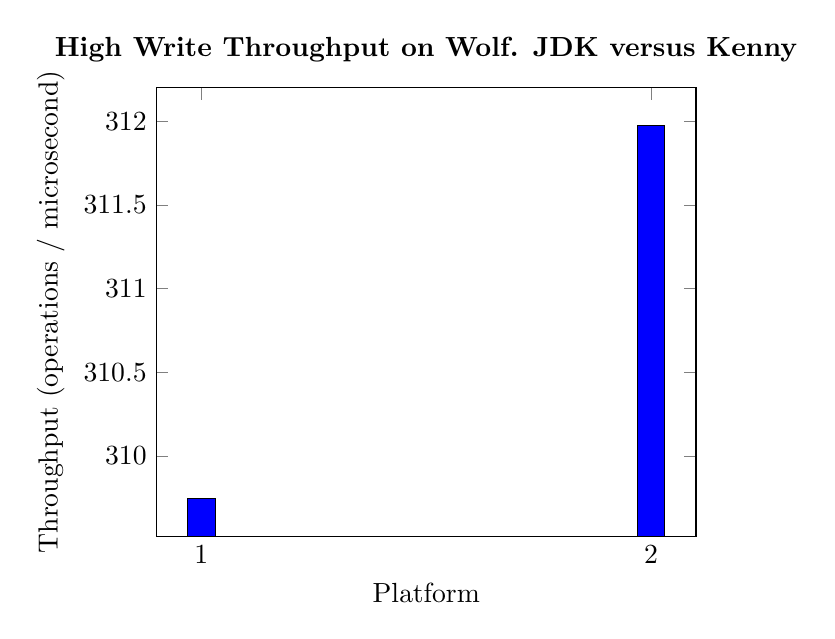
\begin{tikzpicture}
\begin{axis}[
    symbolic x coords={1,2,3,4},
    xtick=data,xlabel=Platform,ylabel=Throughput (operations / microsecond), title=\textbf{High Write Throughput on Wolf. JDK versus Kenny}]
    \addplot[ybar,fill=blue] coordinates {
        (1,309.743)
        (2,311.976)
    };
\end{axis}
\end{tikzpicture}
\vspace{1cm}\\
1: My Structure\\
2: JDK Structure\\

\end{document}
